\newpage
\chaptertitle{CHAPTER 4: RESULTS AND DISCUSSION}
\label{chap:results-discussion}

\subheading{4.1 INTRODUCTION}
\label{sec:results-introduction}

\fontsize{12}{14}\selectfont

This chapter presents the observed implementation evidence for NexRag and discusses the system strictly on the basis of repository artefacts and local verification carried out on \textbf{3 April 2026}. The emphasis is on reproducible evidence such as service status, indexed-document counts, test-script output, query logs, and sample retrieval results. This approach avoids unsupported claims while still allowing a meaningful assessment of the system as a hybrid academic assistant.

\subheading{4.2 IMPLEMENTATION ENVIRONMENT}
\label{sec:results-environment}

NexRag is implemented as a local full-stack application. The backend depends on Python, the frontend on the Node-Vite toolchain, and the graph service on Java for Apache Jena Fuseki. The local environment observed during verification is summarized in Table 4.1.

\begin{center}
\normalsize \textbf{\textit{Table 4.1: Repository Verification Summary}}
\end{center}

\begingroup
\footnotesize
\renewcommand{\arraystretch}{1.12}
\setlength{\tabcolsep}{4pt}
\begin{table}[H]
\centering
\label{tab:repository-verification}
\begin{tabularx}{\textwidth}{|>{\RaggedRight\arraybackslash\hspace{0pt}}X|>{\RaggedRight\arraybackslash\hspace{0pt}}X|>{\RaggedRight\arraybackslash\hspace{0pt}}X|}
\hline
\textbf{Item} & \textbf{Observed Result} & \textbf{Interpretation} \\ \hline
Python runtime & 3.10.11 & Backend requirement satisfied \\ \hline
Node runtime & v24.11.1 & Frontend toolchain available \\ \hline
Java runtime & OpenJDK 17.0.17 & Compatible with Fuseki \\ \hline
API status snapshot & 7 PDFs, 290 chunks, vector ready, local model present & Retrieval pipeline configured \\ \hline
Router test & Passed & Intent rules operational \\ \hline
Retrieval test & Passed model and interface checks & Retrieval subsystem loads correctly \\ \hline
KG test & Passed against live endpoint & Graph retrieval path verified through Fuseki \\ \hline
Frontend build & Passed & Production frontend bundle generated successfully \\ \hline
\end{tabularx}
\end{table}
\endgroup

The observed configuration matches the intended local-first design described in the repository. During local validation, the backend, retrieval stack, graph service, and local model were all available, which allowed both knowledge-graph mode and combined-mode responses to be verified directly from the running application.

\subheading{4.3 INDEXED KNOWLEDGE SOURCES}
\label{sec:results-indexed-sources}

The document corpus available in the repository consists of seven PDFs and an indexed chunk store containing 290 chunks. These files represent the knowledge base used by the retrieval engine for academic assistance.

\begin{center}
\normalsize \textbf{\textit{Table 4.2: Current Indexed Document Collection}}
\end{center}

\begingroup
\footnotesize
\renewcommand{\arraystretch}{1.12}
\setlength{\tabcolsep}{4pt}
\begin{table}[H]
\centering
\label{tab:indexed-document-collection}
\begin{tabularx}{\textwidth}{|>{\RaggedRight\arraybackslash\hspace{0pt}}p{0.10\textwidth}|>{\RaggedRight\arraybackslash\hspace{0pt}}X|>{\RaggedRight\arraybackslash\hspace{0pt}}X|}
\hline
\textbf{Sl. No.} & \textbf{Document Name} & \textbf{Observed Role} \\ \hline
1 & \path|2309.17288v3.pdf| & Technical or research reference \\ \hline
2 & \path|Circular_TechFest.pdf| & Institutional circular content \\ \hline
3 & \path|CSE_Syllabus_S5.pdf| & Course and syllabus information \\ \hline
4 & \path|Guidelines-Format_for_Project_Report.pdf| & Project-report formatting guidance \\ \hline
5 & \path|KTU_Handbook_2024.pdf| & Regulation and academic handbook source \\ \hline
6 & \path|Seminar Guidelines.pdf| & Seminar process and format guidance \\ \hline
7 & \path|Tips for good Presentation .pdf| & Presentation support material \\ \hline
\end{tabularx}
\end{table}
\endgroup

The repository also contains Turtle files such as \path|mesitam_data.ttl|, \path|university_faq.ttl|, and \path|merged_kg.ttl|. Inspection of these files shows graph entities for departments, faculty, courses, and regulations, confirming that the graph layer is structurally meaningful and actively queryable through the live Fuseki endpoint observed during validation.

The composition of the corpus is itself important for interpreting system behavior. The indexed set is not a random collection of documents; it contains precisely the kinds of artefacts that dominate routine academic queries, including handbook regulations, seminar instructions, project-format guidance, and syllabus files. This alignment between corpus content and user intent explains why the retriever performs well on attendance and seminar-related questions. It also indicates that further gains in answer coverage are likely to come more from corpus expansion and graph enrichment than from major architectural change.

\subheading{4.4 FUNCTIONAL VERIFICATION}
\label{sec:results-functional-verification}

Functional verification was performed using the repository's own test scripts. The import and status tests confirmed successful loading of the backend modules and reported seven PDFs, 290 chunks, vector readiness, and an available local model. The router test passed its provided cases, indicating that the rule-based intent categories are functioning as intended for the covered examples.

The retrieval test confirmed that the embedding model, reranker, and retrieval interfaces load correctly. The graph service was also reachable during validation, and direct API queries such as ``Who teaches Computer Graphics?'' and ``What is the minimum attendance rule?'' returned structured graph evidence together with routed responses. The verification therefore supports both the operational state of the retrieval subsystem and the live readiness of the graph subsystem.

From an engineering standpoint, these outcomes show that the project is beyond the stage of a static code demonstration. The router, retriever, metadata store, and model interface are integrated sufficiently to support verifiable end-to-end query handling on the document side. At the same time, the graph-service dependency remains visible as a real operational condition rather than being hidden. This is a useful result because it reveals the actual deployment boundary of the system and clarifies which components require process-level management in a production-like setup.

\subheading{4.5 ROUTING AND RETRIEVAL OUTCOMES}
\label{sec:results-routing-retrieval}

Direct query checks were used to observe practical behavior on representative academic questions. Table 4.3 summarizes the route labels associated with three typical inputs.

\begin{center}
\normalsize \textbf{\textit{Table 4.3: Sample Query Routing Outcomes}}
\end{center}

\begingroup
\footnotesize
\renewcommand{\arraystretch}{1.12}
\setlength{\tabcolsep}{4pt}
\begin{table}[H]
\centering
\label{tab:routing-outcomes}
\begin{tabularx}{\textwidth}{|>{\RaggedRight\arraybackslash\hspace{0pt}}X|>{\RaggedRight\arraybackslash\hspace{0pt}}X|>{\RaggedRight\arraybackslash\hspace{0pt}}X|}
\hline
\textbf{Query} & \textbf{Detected Intent} & \textbf{Primary Evidence Path} \\ \hline
Who teaches Computer Graphics? & \path|FACULTY_INFO| & Knowledge graph \\ \hline
What is the minimum attendance rule? & \path|REGULATION| & Document retrieval \\ \hline
Explain seminar guidelines & \path|DEFINITION| & Document retrieval \\ \hline
\end{tabularx}
\end{table}
\endgroup

For the query ``What is the minimum attendance rule?'', the top retrieval result came from \path|KTU_Handbook_2024.pdf| with a relevance score near \textbf{0.9663}. The returned passage explicitly stated the minimum attendance requirement and condonation condition, indicating a strong policy match. For the query ``Explain seminar guidelines'', the highest-ranked results were drawn from \path|Guidelines-Format_for_Project_Report.pdf| and \path|Seminar Guidelines.pdf|, showing that the retriever can locate both closely related procedural and seminar-specific content. The results are summarized in Table 4.4.

\begin{center}
\normalsize \textbf{\textit{Table 4.4: Sample Retrieval Outputs and Relevance Scores}}
\end{center}

\begingroup
\footnotesize
\renewcommand{\arraystretch}{1.12}
\setlength{\tabcolsep}{4pt}
\begin{table}[H]
\centering
\label{tab:retrieval-outputs}
\begin{tabularx}{\textwidth}{|>{\RaggedRight\arraybackslash\hspace{0pt}}X|>{\RaggedRight\arraybackslash\hspace{0pt}}X|>{\RaggedRight\arraybackslash\hspace{0pt}}p{0.10\textwidth}|>{\RaggedRight\arraybackslash\hspace{0pt}}p{0.10\textwidth}|>{\RaggedRight\arraybackslash\hspace{0pt}}X|}
\hline
\textbf{Query} & \textbf{Top Source} & \textbf{Page} & \textbf{Score} & \textbf{Observation} \\ \hline
What is the minimum attendance rule? & \path|KTU_Handbook_2024.pdf| & 1 & 0.9663 & Strong direct policy match \\ \hline
What is the minimum attendance rule? & \path|KTU_Handbook_2024.pdf| & N/A & 0.2770 & Secondary supporting passage \\ \hline
Explain seminar guidelines & \path|Guidelines-Format_for_Project_Report.pdf| & 1 & 0.9485 & High-level procedural guidance \\ \hline
Explain seminar guidelines & \path|Seminar Guidelines.pdf| & 1 & 0.8702 & Seminar-specific evidence \\ \hline
Explain seminar guidelines & \path|Seminar Guidelines.pdf| & N/A & 0.6865 & Additional supporting detail \\ \hline
\end{tabularx}
\end{table}
\endgroup

These results indicate that the retrieval engine is effective when the query aligns with the indexed academic corpus. They also show the value of reranking, because related documents compete for top positions in procedural queries.

The sample outputs also illustrate the complementary roles of dense and lexical evidence. The attendance-rule query benefits from exact policy wording, which naturally favours handbook passages containing formal regulatory language. The seminar-guideline query, by contrast, is broader and therefore returns multiple relevant procedural documents that must be ordered by semantic closeness and contextual usefulness. This difference is consistent with the motivation for combining BM25, vector retrieval, and reranking within a single pipeline.

\subheading{4.6 INTERFACE AND WORKFLOW}
\label{sec:results-interface-workflow}

The frontend implementation reveals a user-oriented design. The application provides a welcome state with prompt suggestions, a streaming chat view, route badges, source evidence, a system-status panel, and a knowledge-graph editor. These interface choices are important because they expose the reasoning path of the system instead of presenting the answer as a black box.

\begin{figure}[H]
\centering
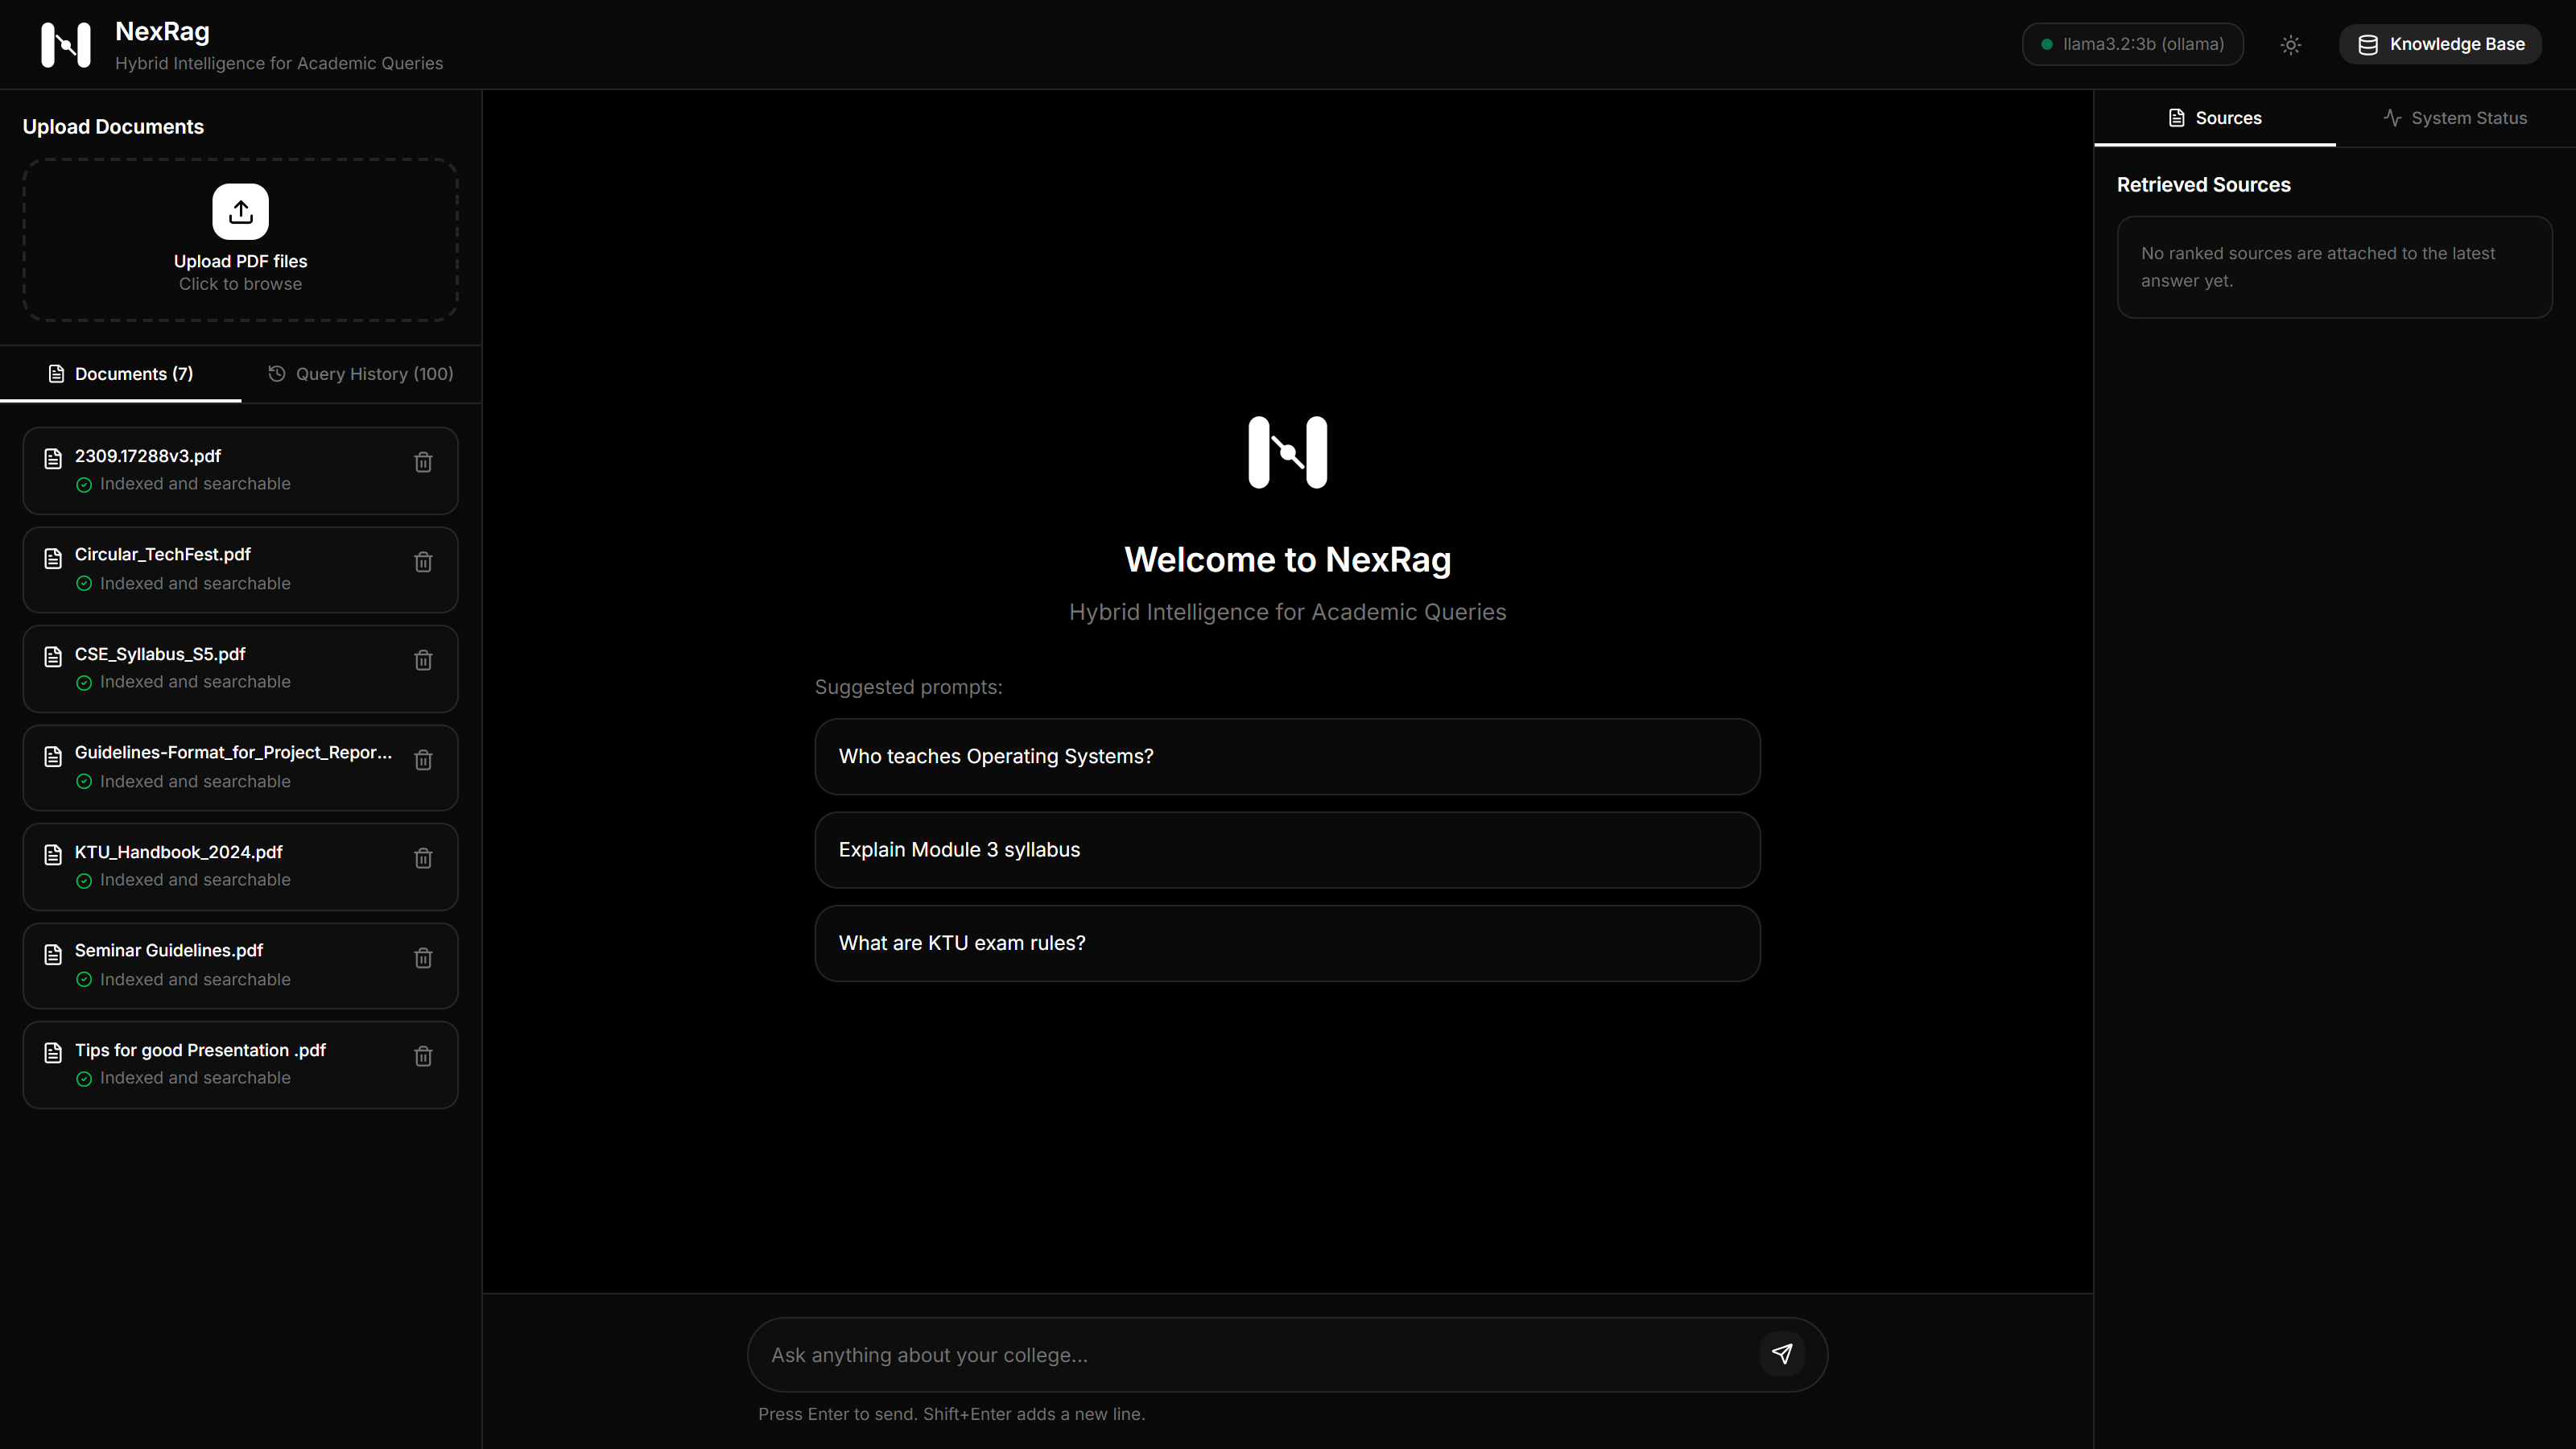
\includegraphics[width=\textwidth]{nexrag_main_ui.png}
\label{fig:nexrag-main-ui}
\vspace{-0.25cm}
\begin{center}
\normalsize \textbf{\textit{Fig4.1. Main User Interface of the NexRag Frontend}}
\end{center}
\end{figure}

\begin{figure}[H]
\centering
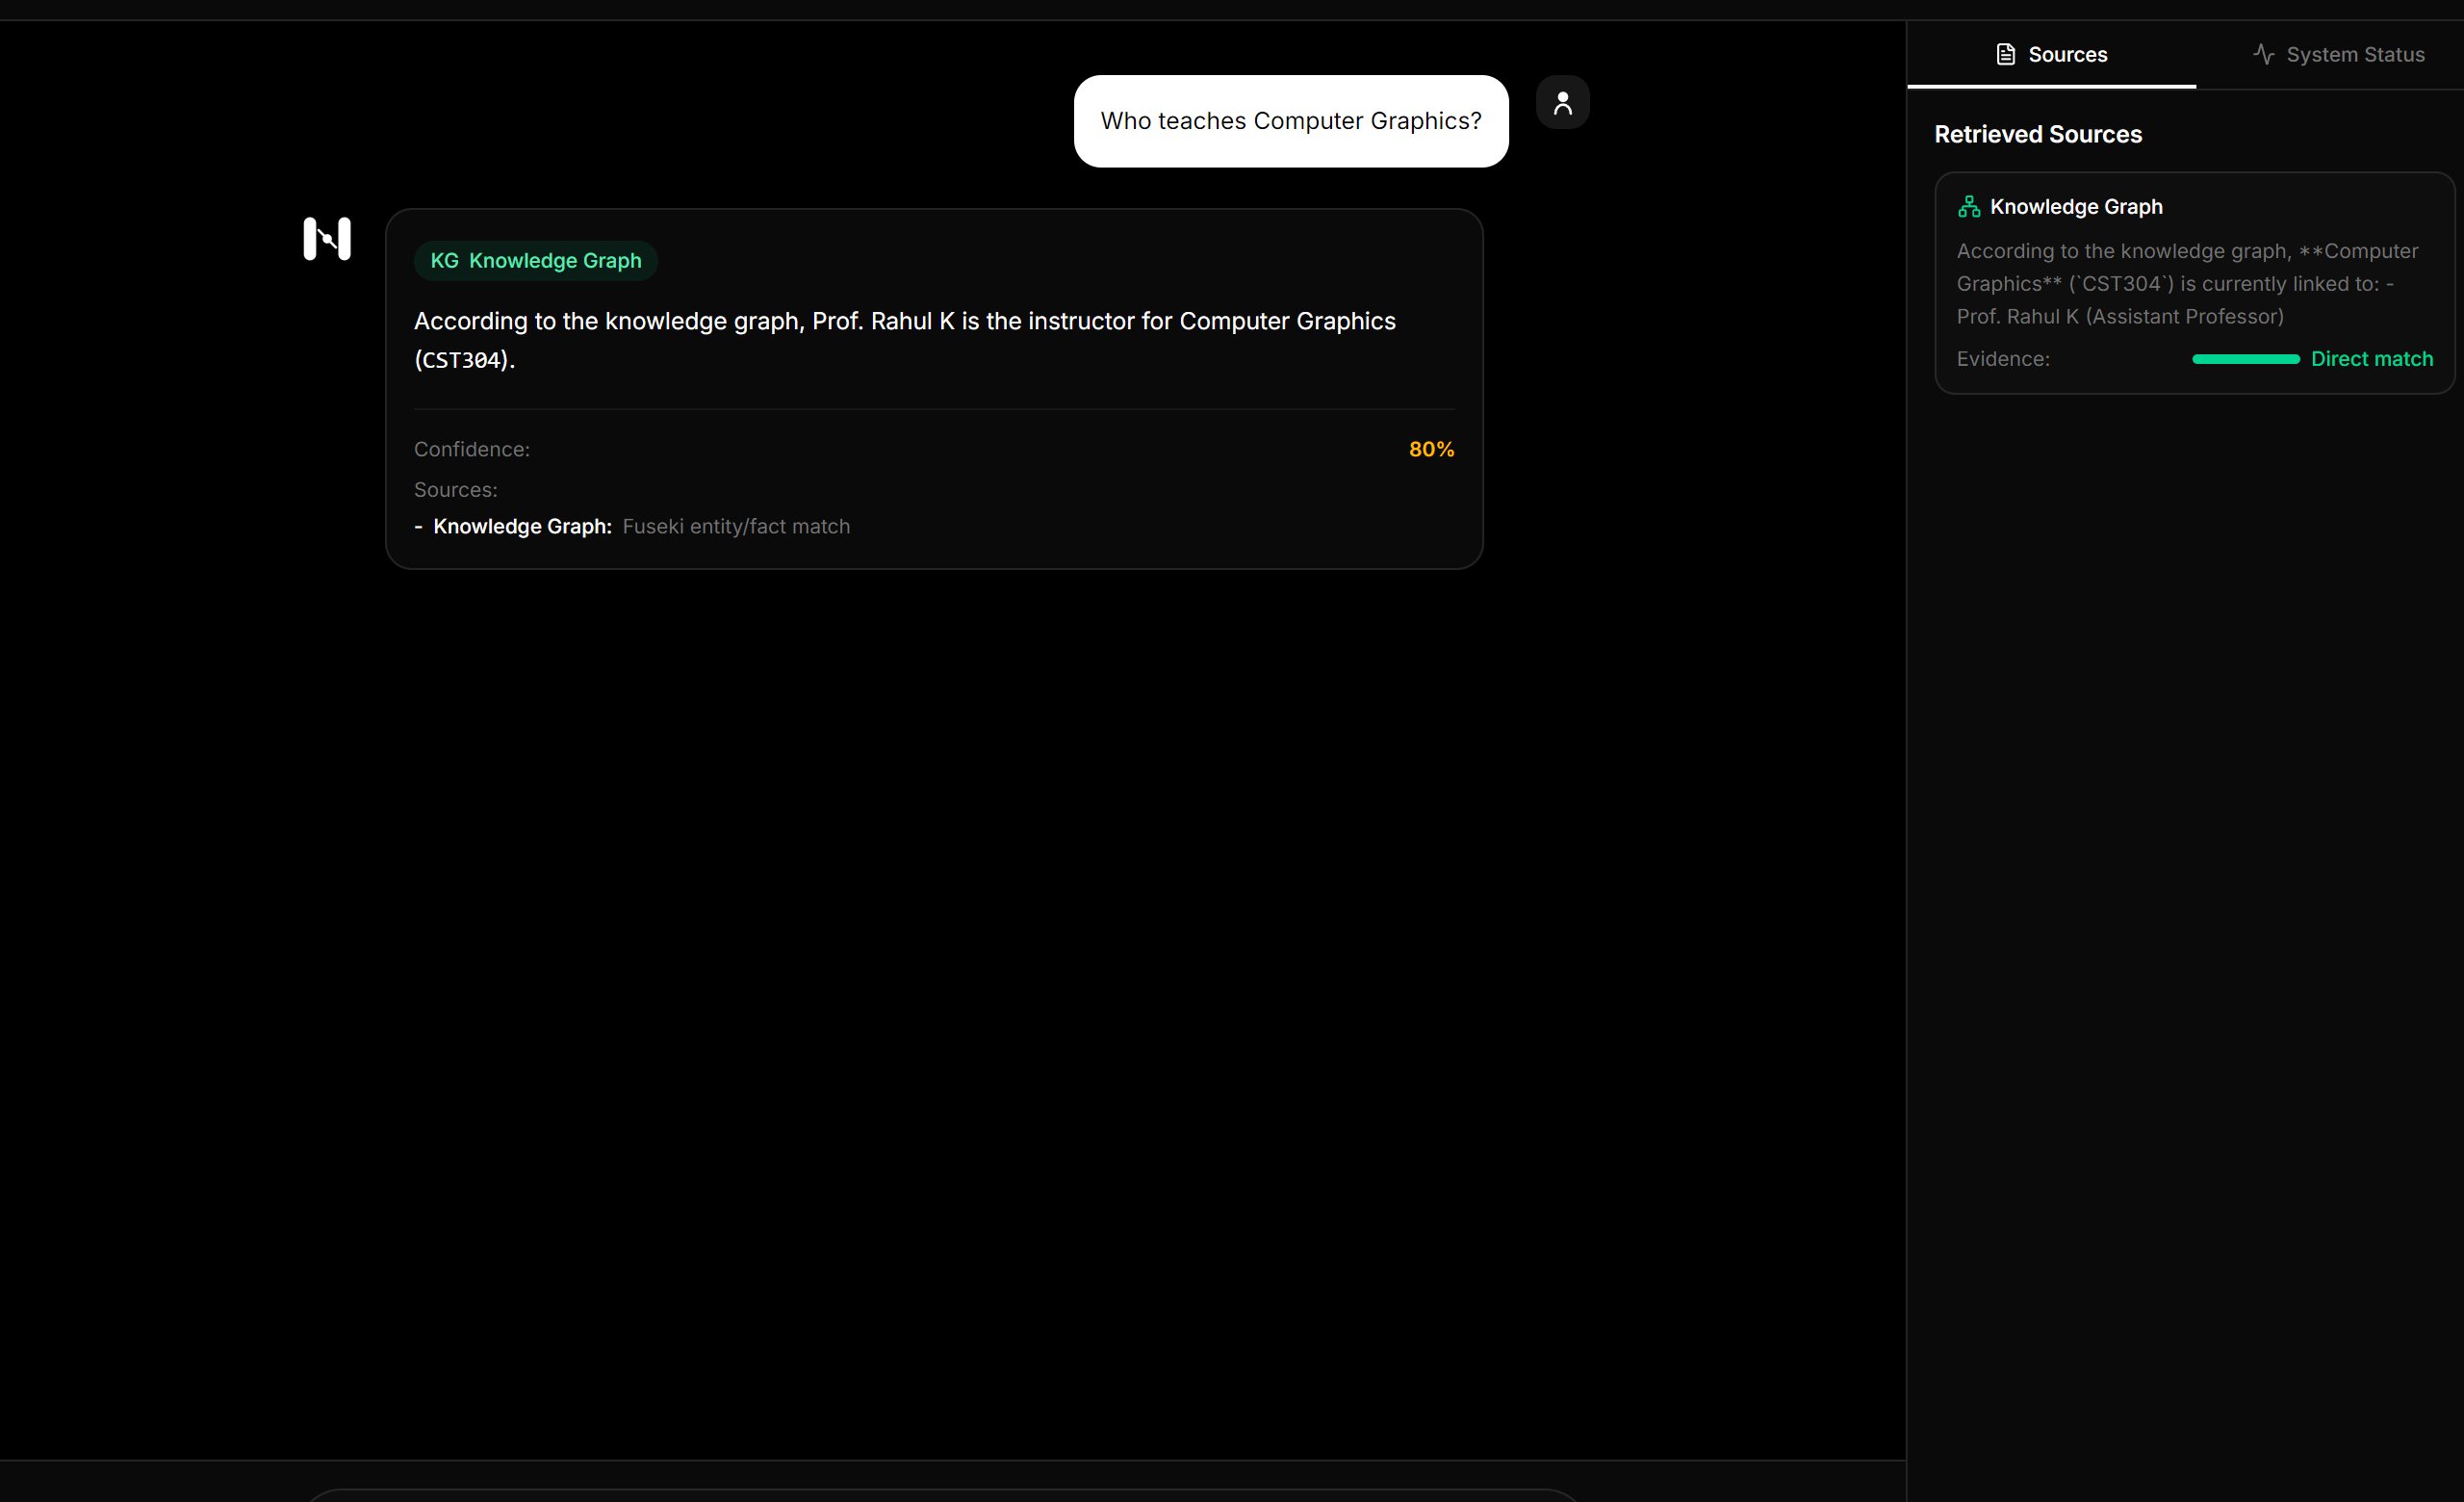
\includegraphics[width=\textwidth]{nexrag_streaming_answer_crop.png}
\label{fig:nexrag-streaming-answer}
\vspace{-0.25cm}
\begin{center}
\normalsize \textbf{\textit{Fig4.2. Streaming Answer View with Routing and Source Evidence}}
\end{center}
\end{figure}

\begin{figure}[H]
\centering
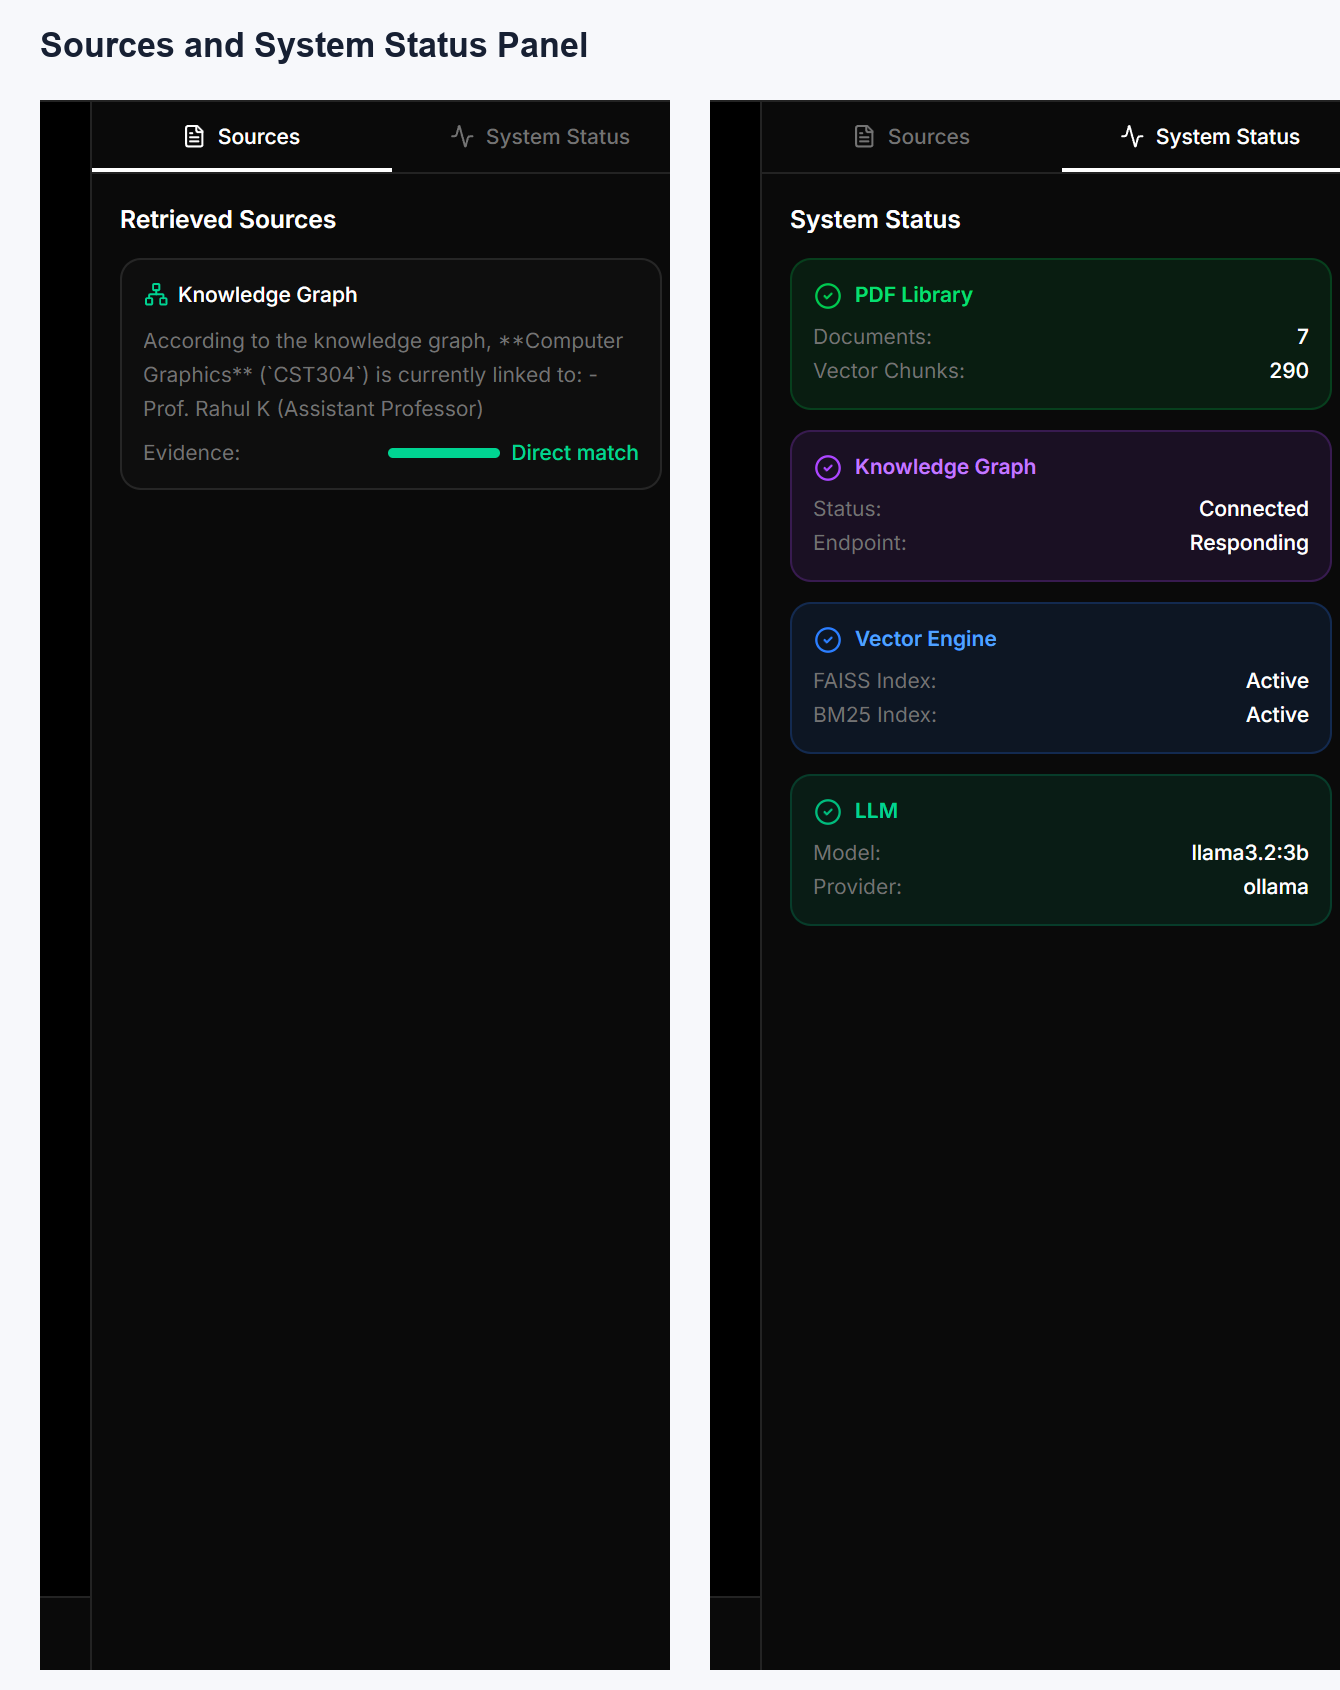
\includegraphics[width=0.78\textwidth]{nexrag_sources_panel.png}
\label{fig:nexrag-sources-panel}
\vspace{-0.25cm}
\begin{center}
\normalsize \textbf{\textit{Fig4.3. Intelligence Panel Showing Retrieved Sources and System Status}}
\end{center}
\end{figure}

\begin{figure}[H]
\centering
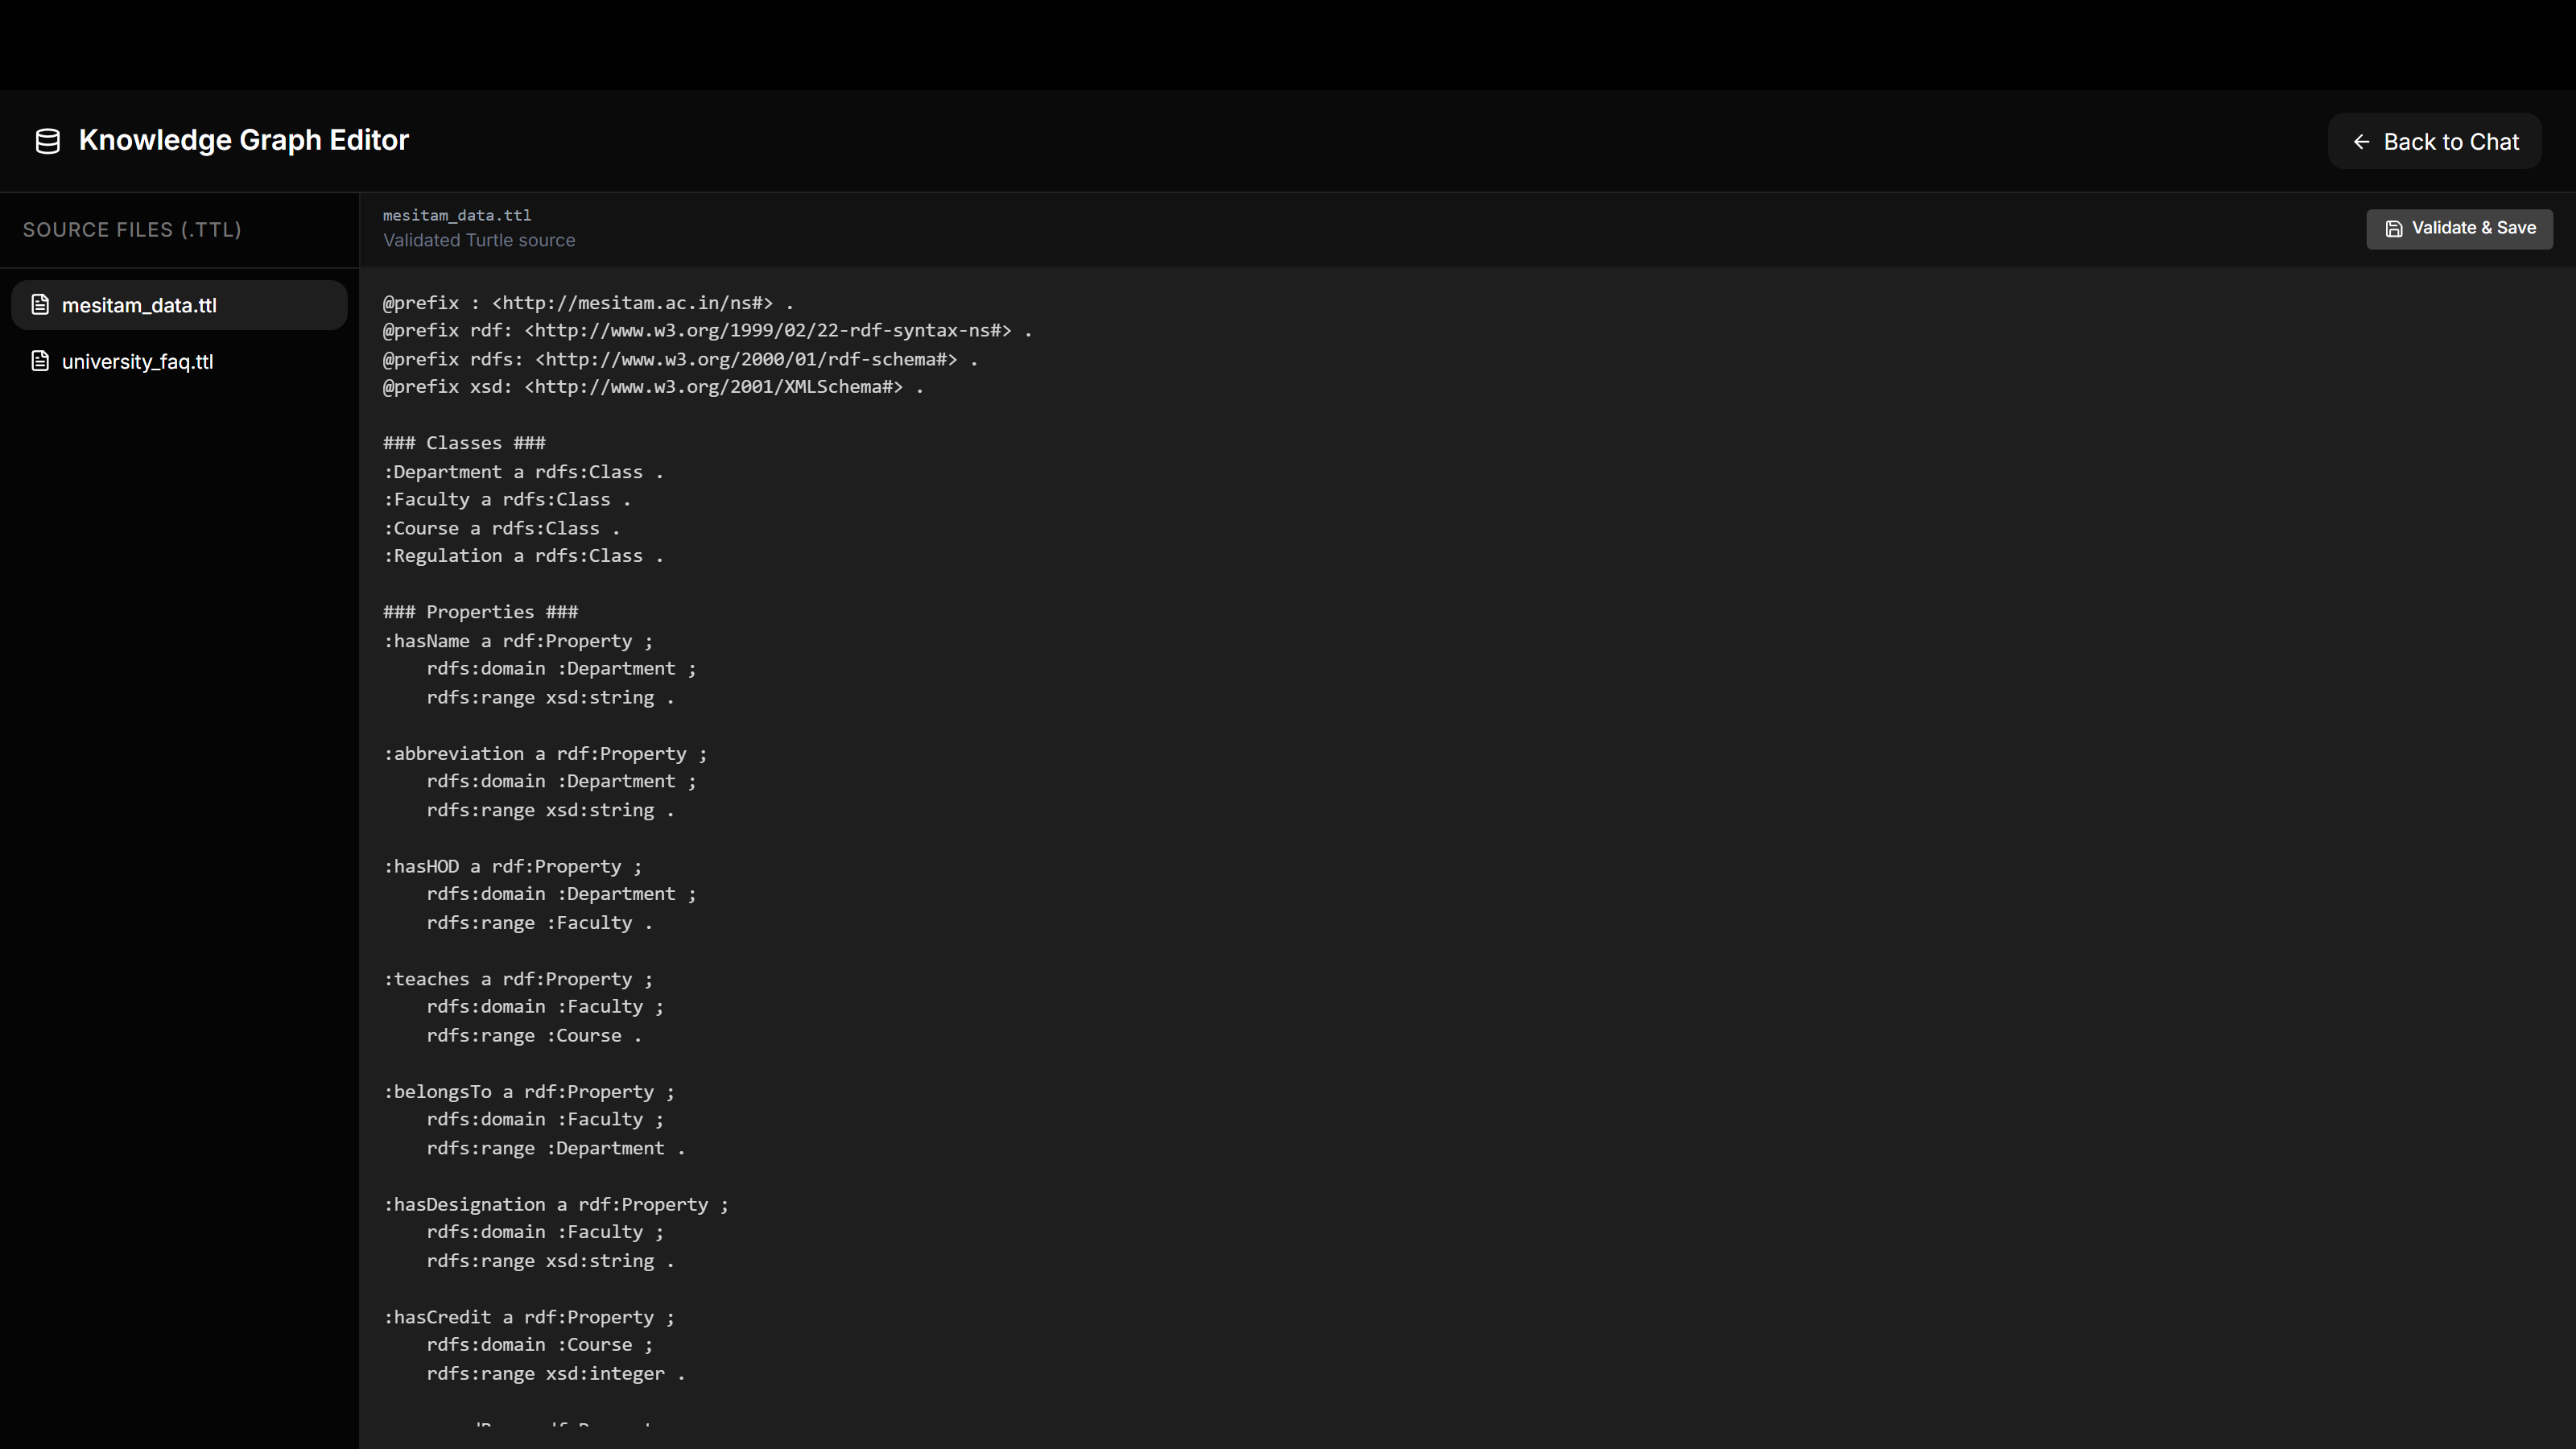
\includegraphics[width=\textwidth]{nexrag_kg_editor.png}
\label{fig:nexrag-kg-editor}
\vspace{-0.25cm}
\begin{center}
\normalsize \textbf{\textit{Fig4.4. Knowledge Graph Editor Interface for Turtle File Update}}
\end{center}
\end{figure}

From an evaluation perspective, these interface elements are meaningful because they improve interpretability. Users can determine whether an answer came from graph evidence, document evidence, or a combined route, and can inspect the supporting sources directly.

\subheading{4.7 PERFORMANCE ANALYSIS}
\label{sec:results-performance}

The repository's query-history log provides limited but useful latency observations. Two recorded examples showed response times of \textbf{13.87 seconds} for ``What is RAG?'' and \textbf{11.18 seconds} for ``Who teaches CS301?''. These values are not sufficient for statistical benchmarking, but they are consistent with a local RAG pipeline that includes retrieval and language-model generation.

\begin{center}
\normalsize \textbf{\textit{Table 4.5: Observed Query Log Characteristics}}
\end{center}

\begingroup
\footnotesize
\renewcommand{\arraystretch}{1.12}
\setlength{\tabcolsep}{4pt}
\begin{table}[H]
\centering
\label{tab:query-log-characteristics}
\begin{tabularx}{\textwidth}{|>{\RaggedRight\arraybackslash\hspace{0pt}}X|>{\RaggedRight\arraybackslash\hspace{0pt}}p{0.15\textwidth}|>{\RaggedRight\arraybackslash\hspace{0pt}}p{0.14\textwidth}|>{\RaggedRight\arraybackslash\hspace{0pt}}X|}
\hline
\textbf{Logged Query} & \textbf{Intent} & \textbf{Latency (s)} & \textbf{Observed Response Character} \\ \hline
What is RAG? & \path|DEFINITION| & 13.87 & Explanatory answer from retrieved context \\ \hline
Who teaches CS301? & \path|GENERAL| & 11.18 & Uncertain output due weak evidence at that time \\ \hline
\end{tabularx}
\end{table}
\endgroup

The retrieval results also indicate that the ranking pipeline is functioning well for high-signal queries. The attendance-rule query returned a highly relevant handbook passage, while seminar-related queries retrieved multiple appropriate procedural sources. This suggests that the combined dense, sparse, and reranking strategy is suitable for the current corpus, though larger-scale testing would be needed for stronger conclusions.

These latency observations should be interpreted in relation to the deployment model. NexRag prioritizes local execution, grounded prompting, and source transparency over raw response speed. In a small institutional installation this is an acceptable trade-off because queries are typically low-volume and correctness is more important than sub-second interaction. Nevertheless, the current figures also suggest where optimization effort should be concentrated in future work, particularly in graph-service orchestration, reranking efficiency, and prompt length management.

\begin{figure}[H]
\centering
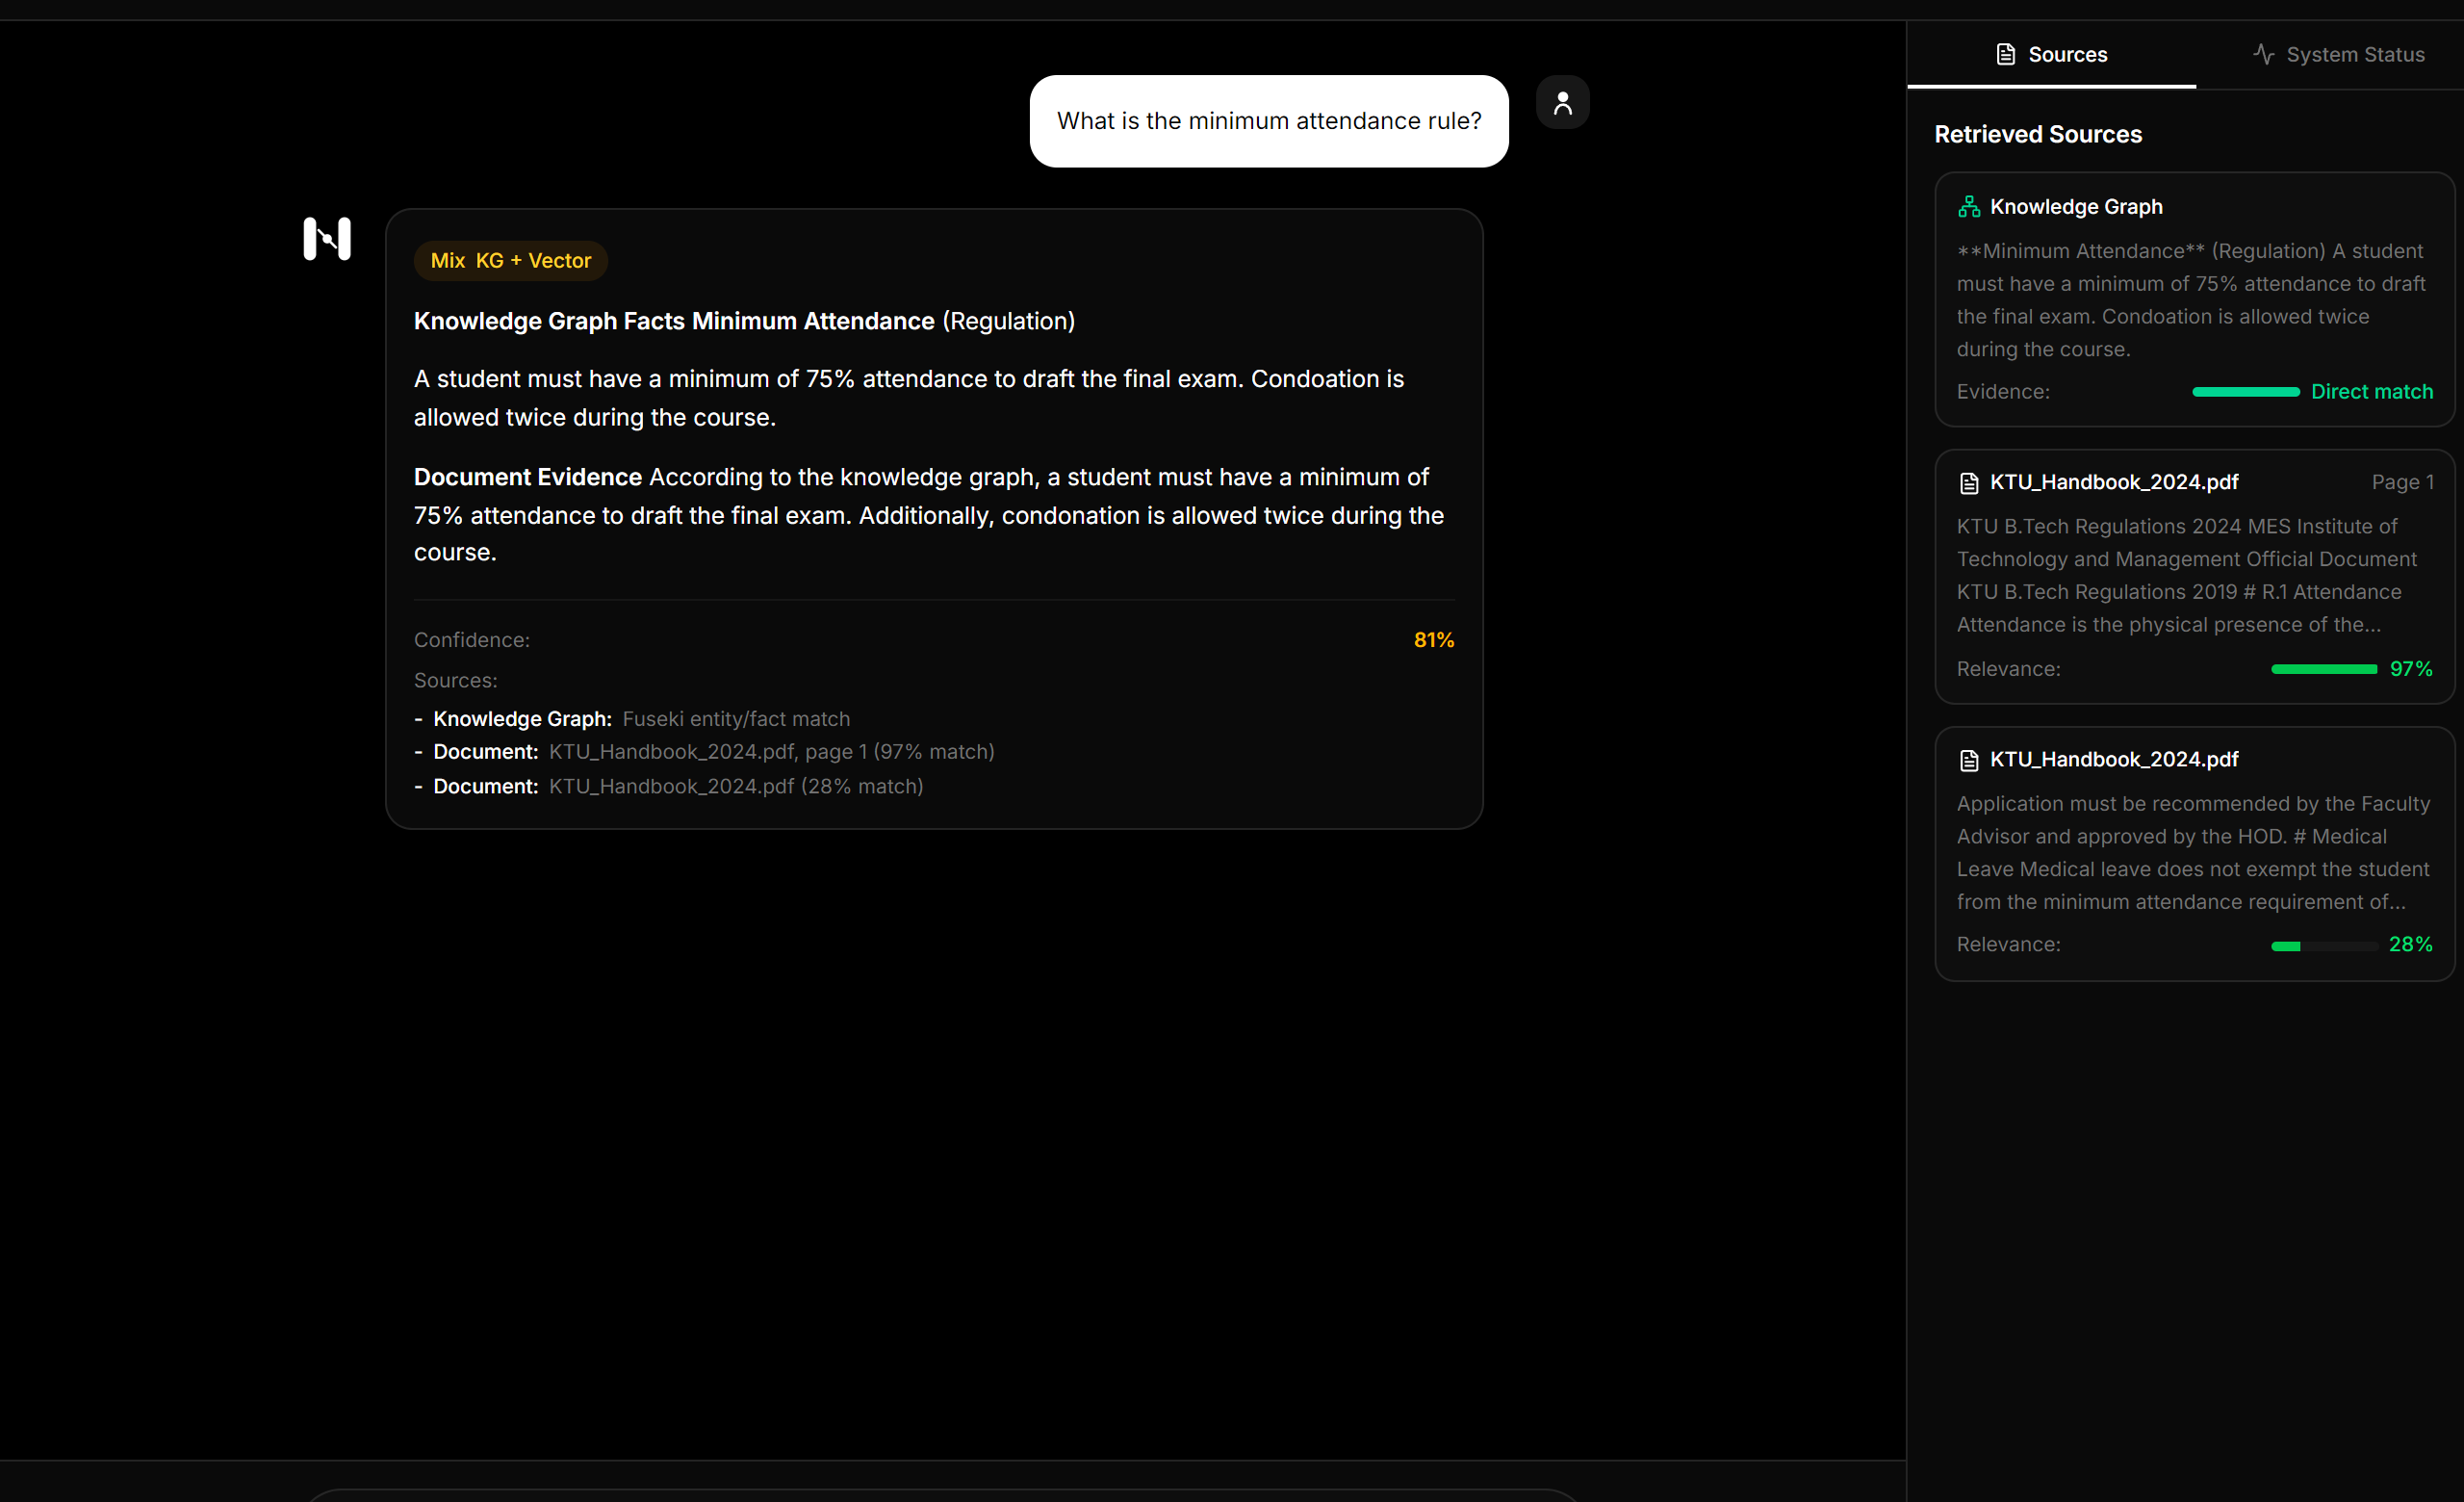
\includegraphics[width=\textwidth]{nexrag_query_attendance_crop.png}
\label{fig:nexrag-query-attendance}
\vspace{-0.25cm}
\begin{center}
\normalsize \textbf{\textit{Fig4.5. Retrieval Output for an Attendance Rule Query}}
\end{center}
\end{figure}

\begin{figure}[H]
\centering
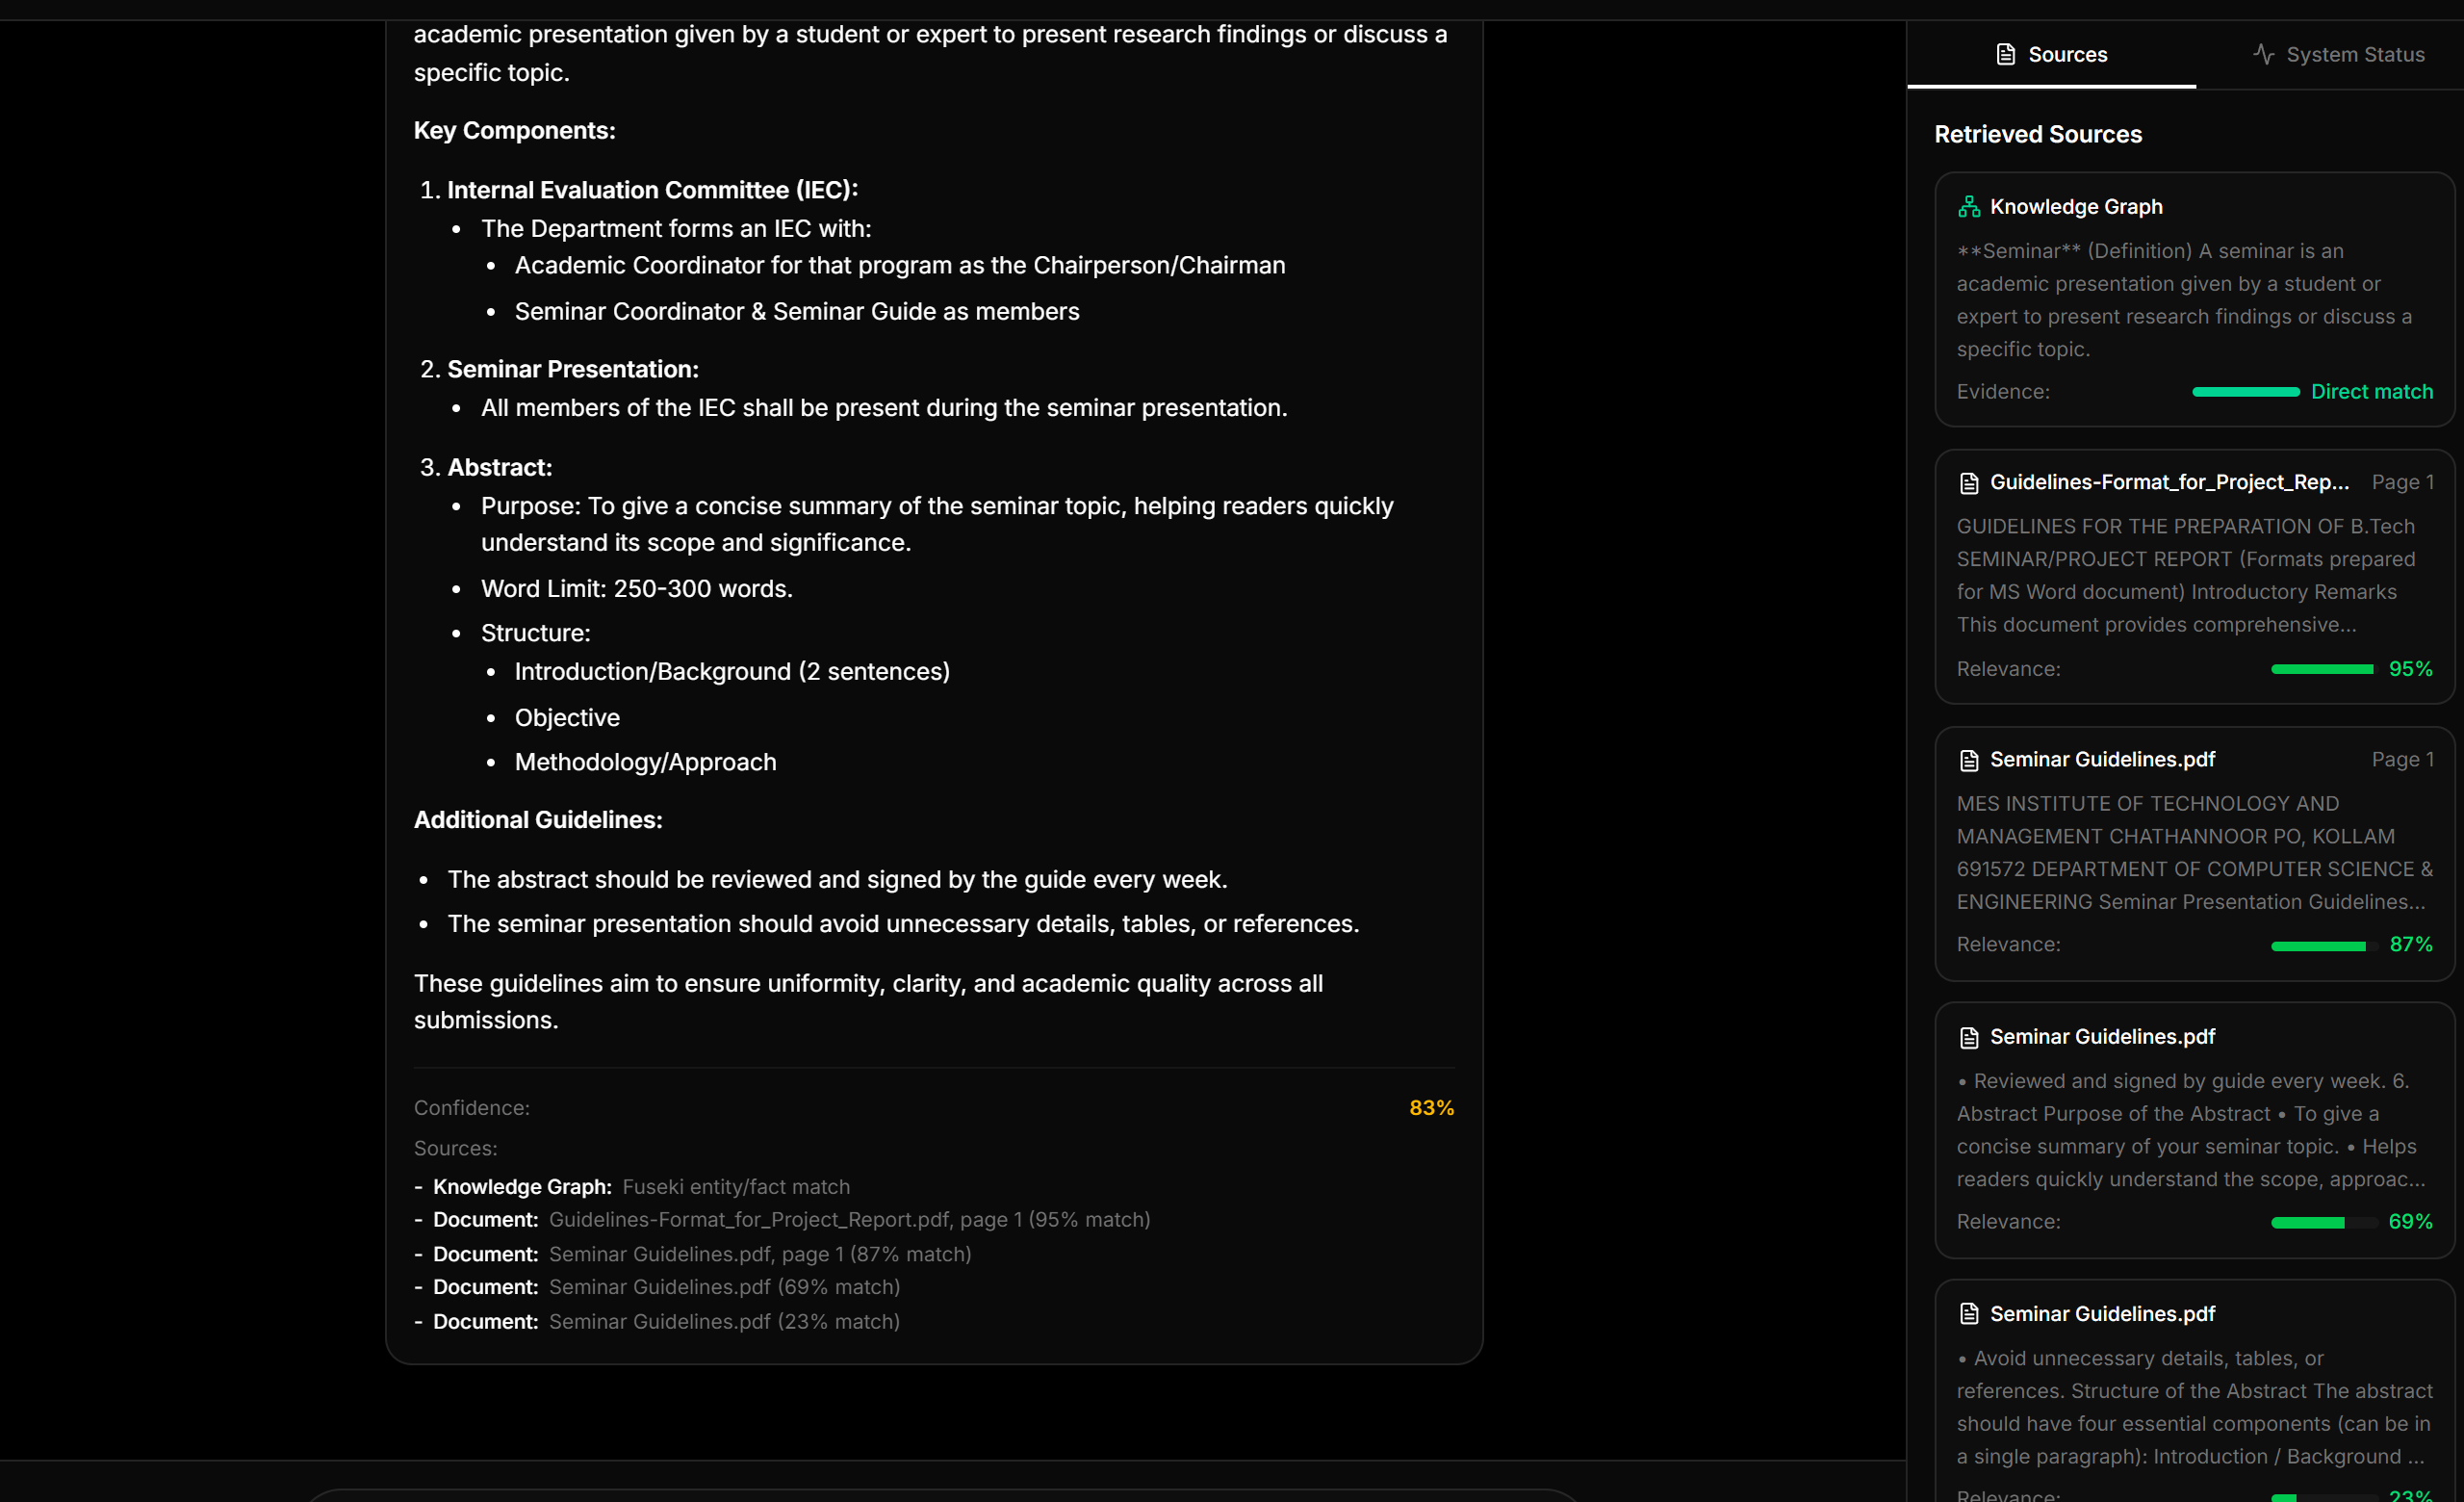
\includegraphics[width=\textwidth]{nexrag_query_seminar_crop.png}
\label{fig:nexrag-query-seminar}
\vspace{-0.25cm}
\begin{center}
\normalsize \textbf{\textit{Fig4.6. Retrieval Output for a Seminar Guideline Query}}
\end{center}
\end{figure}

\subheading{4.8 OPERATING MODES}
\label{sec:results-operating-modes}

NexRag can operate in four practical modes depending on evidence availability: knowledge-graph mode, vector-search mode, combined mode, and no-hit mode. These modes are summarized in Table 4.6.

\begin{center}
\normalsize \textbf{\textit{Table 4.6: Comparative Discussion of Operating Modes}}
\end{center}

\begingroup
\footnotesize
\renewcommand{\arraystretch}{1.12}
\setlength{\tabcolsep}{4pt}
\begin{table}[H]
\centering
\label{tab:operating-modes}
\begin{tabularx}{\textwidth}{|>{\RaggedRight\arraybackslash\hspace{0pt}}X|>{\RaggedRight\arraybackslash\hspace{0pt}}X|>{\RaggedRight\arraybackslash\hspace{0pt}}X|>{\RaggedRight\arraybackslash\hspace{0pt}}X|}
\hline
\textbf{Mode} & \textbf{Trigger Condition} & \textbf{Strength} & \textbf{Limitation} \\ \hline
Knowledge Graph Mode & Structured fact available & Precise entity-level answer & Limited descriptive depth \\ \hline
Vector Search Mode & Document evidence available & Strong procedural explanation & Weaker explicit relations \\ \hline
Combined Mode & Both graph and document evidence available & Best balance of fact and explanation & Depends on both services \\ \hline
No Retrieval Hit & No reliable supporting evidence & Honest uncertainty handling & No substantive answer \\ \hline
\end{tabularx}
\end{table}
\endgroup

During the observed verification session, the graph service was active, so practical behavior included both pure knowledge-graph answers and combined graph-plus-document responses. This allowed the report to capture live evidence for all three meaningful operating modes other than the no-hit fallback.

This mode-based interpretation is useful because it separates architectural capability from session-specific availability. A hybrid assistant should not be judged only by its best-case path, but by how intelligibly it behaves across changing evidence conditions. NexRag performs reasonably well in this respect because the system can still provide source-backed document answers when the graph service is absent, and the interface is designed to expose that operating condition rather than conceal it.

\begin{figure}[H]
\centering
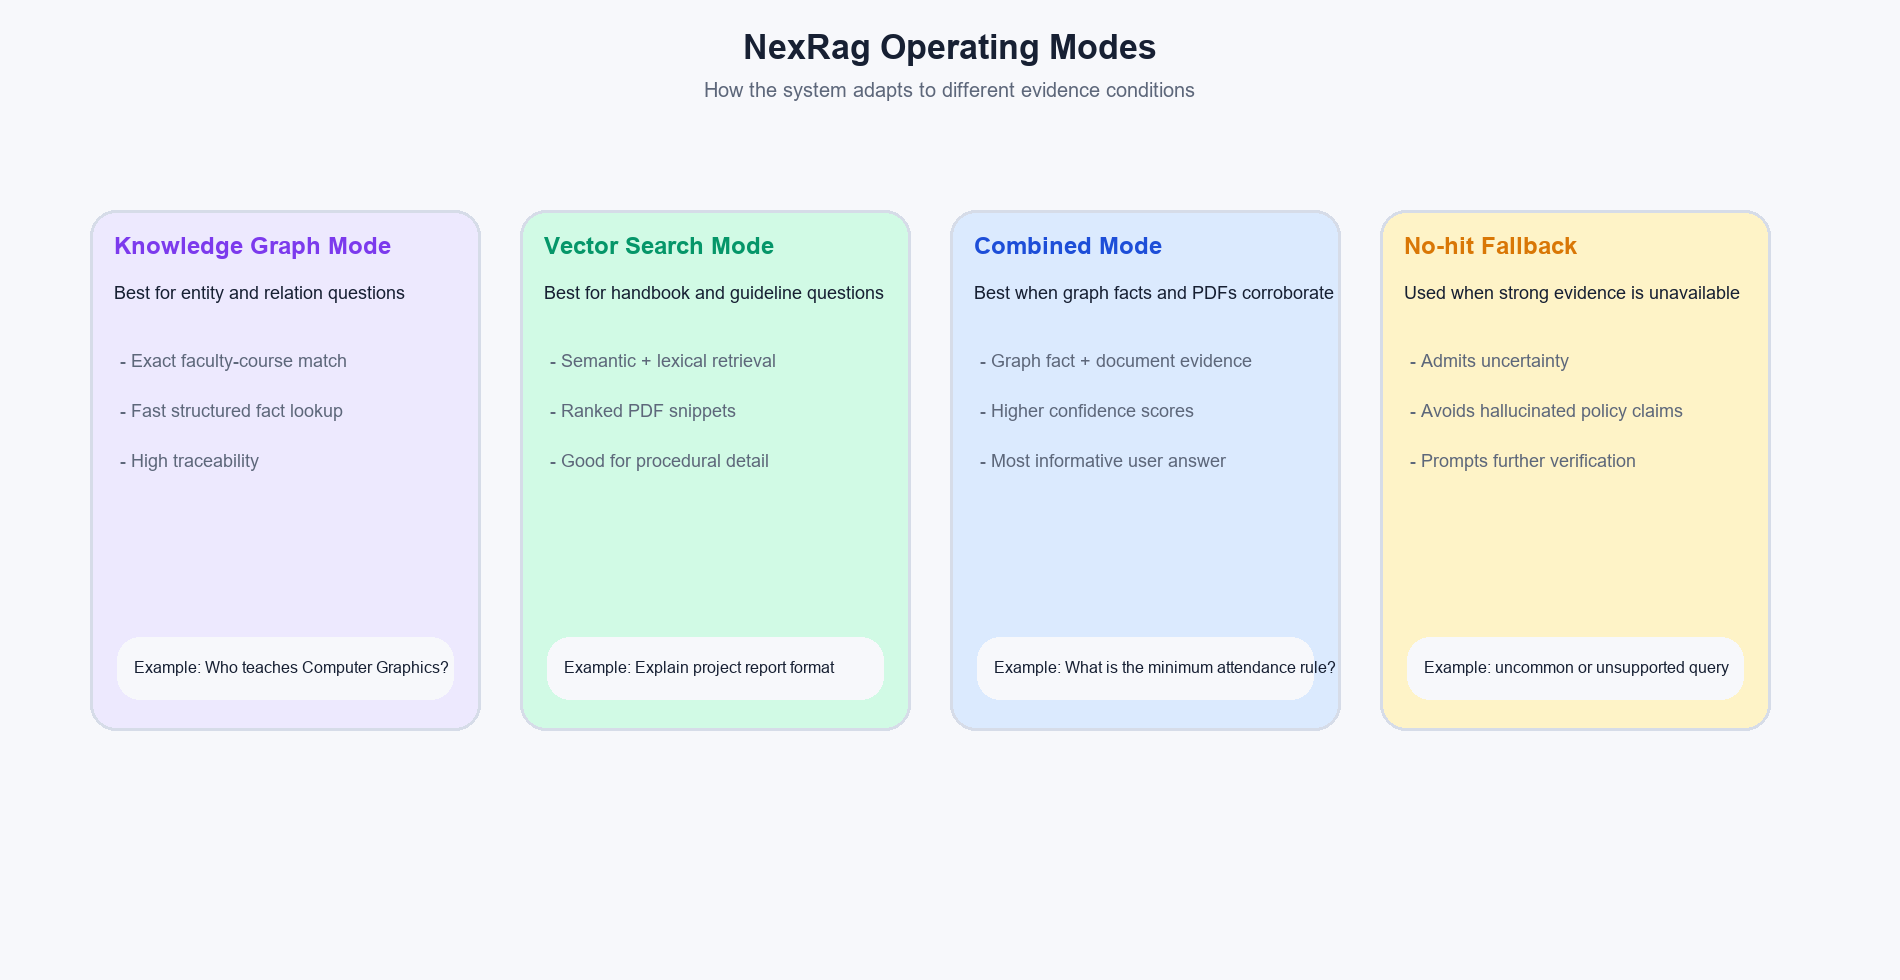
\includegraphics[width=\textwidth]{nexrag_mode_comparison.png}
\label{fig:nexrag-mode-comparison}
\vspace{-0.25cm}
\begin{center}
\normalsize \textbf{\textit{Fig4.7. Comparative Mode Analysis of KG, Vector, and Combined Responses}}
\end{center}
\end{figure}

\subheading{4.9 EVALUATION LIMITATIONS}
\label{sec:results-limitations}

The present evaluation has clear limits. Although the live stack was available during validation, the number of representative queries observed was still small, the latency discussion relies on a short interaction history, and the system has not yet been tested through a long-running institutional deployment or a formal user study. In addition, the report evaluates the current local corpus and graph contents, so answer quality will continue to depend on document freshness and graph completeness.

Despite these constraints, the available evidence supports the central claim of the project: NexRag is a coherent hybrid academic assistant with a working document-retrieval pipeline, a structured graph layer, a local generation path, and an interface designed for evidence visibility. The current results therefore demonstrate feasibility and functional readiness, while also indicating the next steps needed for deployment-grade validation.

In summary, the present evaluation is best understood as a functional verification study rather than a full-scale benchmark. Within that scope, the system demonstrates meaningful capability: relevant academic documents are indexed and retrieved, route decisions are produced, evidence is surfaced to the user, and the local-generation path operates over retrieved context. These are strong indicators that the proposed architecture is technically sound and suitable for continued refinement toward institutional deployment.
